\documentclass[/home/greg/Thesis/main/main.tex]{subfiles}

\begin{document}

\graphicspath{{/home/greg/Neutron_star_modelling/LyneSwitchingAnalytic/LyneErrorCalculation/}}

\section{Calculation inconsistency in Lyne 2010}
In this section I present an inconsistency in the argument of \citet{Lyne2010}
regarding two-state spin-downs. They have presented, amonst others, two types
of data which are related: the estimated spin-down values for the two distinct
states, and the magnitude of timing residuals which they claim results from
this switching. For clarity we begin by considering only this data for PSR
B1828-11. 

In the supplementary material for the paper and in a follow up paper 
\citet{Perrera2014}, the authors generate timing residuals to illusrtrate 
agreement with observation. This is done by taking the proposed spin-down
model, a square-wave switching between two value, and numerically integrating twice to 
get the phase. Subtracting a Taylor expansion fit yeilds the phase-residual which
once multiplied by the spin-period produces the timing residual.

\begin{figure}[htb]
\centering
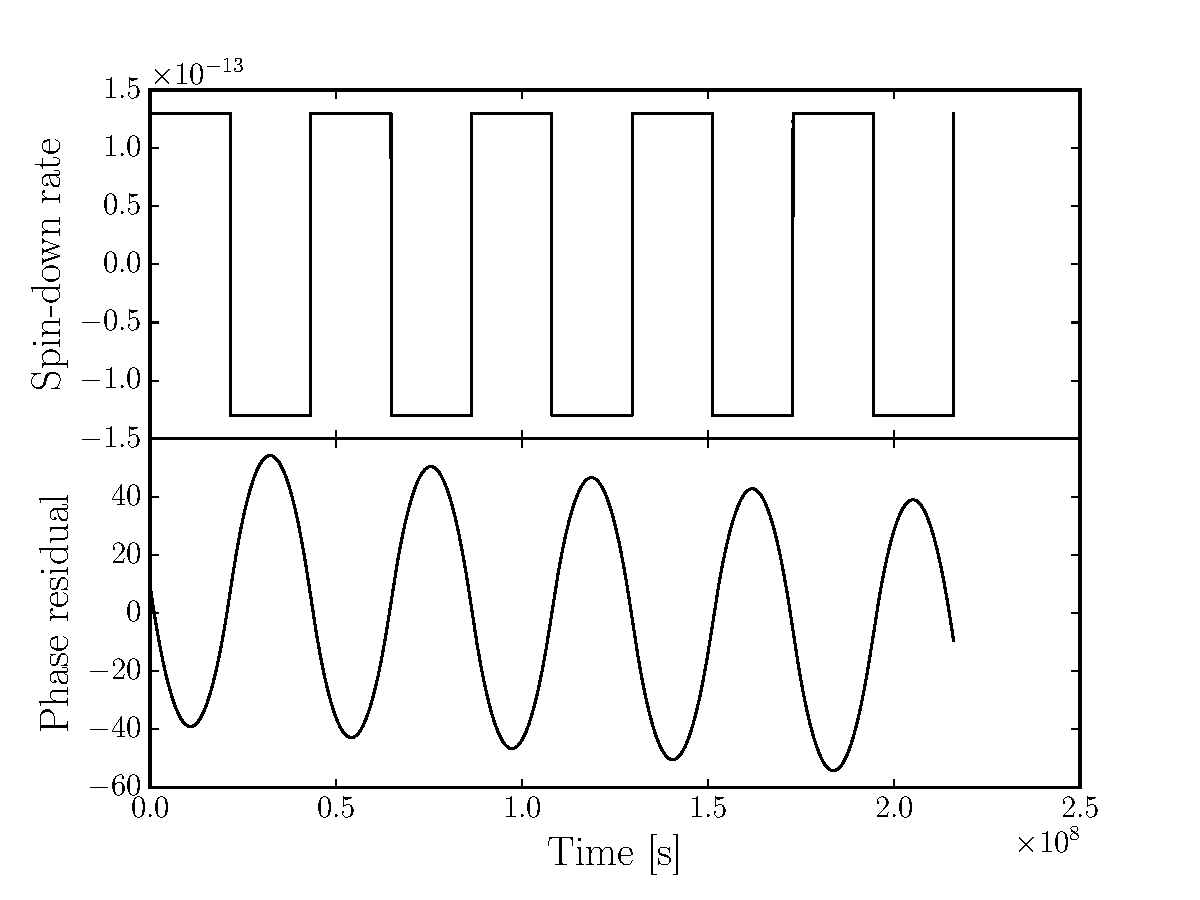
\includegraphics[width=0.5\textwidth]{LyneErrorPlot}
\caption{}
\label{fig:}
\end{figure}

This cannot be done in Tempo because the size of the residual is too large!

\end{document}
